\documentclass[a4paper,10pt]{article}
\usepackage{a4wide,graphicx,enumerate}

\title{Analysis of Euler Solvers for Temperature Equation in Channel Flows}
\author{Girish Nivarti (50951094)}
\date{\today}

\begin{document}
\maketitle

\begin{enumerate}[I]
\item The error norms for each mesh were plotted in Fig.~\ref{norms}. For a mesh 400x160, and $L_2$ norm of $0.0014011$ was found for flux calculation and $9.169\times10^{-6}$ for source calculations. There is a great magnitude difference in these norms, and it is reflected on all mesh sizes. This is perhaps due to the fact that flux calculation requires terms involving temperature field, which adds to the overall error.

\item Both explicit and implicit schemes were used to calculate the solution of the given problem with a fully developed velocity profle, and a fully developed inlflow for temperature. The norms of solution have been plotted for each mesh size, for both implicit (Fig.~\ref{ieOrder}), and explicit (Fig.~\ref{eeOrder}) Euler methods. These plots and with exact values in the following tables, demonstrate that the methods are $2^{nd}$ order accurate. Implicit method was found to converge, to the set convergence criterion of $dT_{max} = 10^{-8}$, in much fewer steps. Despite using a large time step (we will see later that much larger time steps can be taken while using Implicit methods as opposed to Explicit methods), the same values of error norms are arrived at in ~30 times less steps. Something phenomenal! Twice the number of steps (Table.~\ref{normIE} were taken for the time step of 0.1 in the Implicit solution on a 200x80 mesh. The error profile has been plotted (Fig.~\ref{errorprof} for the mesh, errors are similar in both meshes and mimic the fully developed velocity profile everywhere except near the entrance of the channel where the exact profile has been specified at inflow.

\item The efficiency test was conducted, and the relevant features have been tabulated in Table.~\ref{effEE} for explicit scheme, and Table.~\ref{effIE} for implicit method. There was no observable maximum/limiting time step for Implicit scheme. However, as the step size increased beyond certain values, the simulation time went up, iterations up to convergence went up. This is against our intuition as with large time steps we are in effect pacing towards steady state at with bigger leaps, and must reach there sooner. This is not observed for explicit schemes, although the explicit schemes have a much lower maximum time step. This is perhaps due to the approximate factorisation, which gets large values on RHS for large time steps, possibly increasing the maximum change in solution at every iteration. Explicit schemes were simulated using the maximum possible time step which was estimated by experimenting with different possible values of dt.

\item The gradients were calculated for a slightly modified problem (with new boundary conditions on top wall, and a realistic Ec = 0.001). Evidence that the domain size of 25.0 which was chosen for this calculation, has been provided as a plot (Fig.~\ref{size}) of gradient at the bottom wall, with varying channel lengths. These values lie on the same curve that has a global maximum in the region of x = 12.5. Grid convergence study was done, and has been tabulated in Table~\ref{gci}. A final estimate (after using Richardson extrapolation) gives us: $\frac{\partial T}{\partial y}_{max, y = 0} = 1.1291 \pm 6.335 \times 10^{-5} at x = 12.5 \pm 0.006281$. The apparent order of the method was calculated as 1.80881. Plots of the gradient at bottom wall (Fig.~\ref{gradient}), and gradient across the channel (Fig.~\ref{gradientx}) have been drawn for a mesh of size 200x80, and channel length 25.0.


\begin{figure}
  \centering
  \includegraphics[width=0.6\textwidth, angle = -90]{../plots/norm/norm.eps}
  \caption{Norms for flux and source calculations using the finite volume method. Norms ($L_2$) are plotted on a log-log graph with varying cell size (in x direction) as the mesh was refined. The order of accuracy of the method is given by the slope of the line.}
  \label{norms}
\end{figure}

  \begin{table}
      \begin{center}
        \begin{tabular}{|l | l | l | r |}
          \hline
          Mesh Size & $L_2$ Norm & Iterations \\
          \hline
          25x10 & 0.0112145 & 2987 \\
          50x20 & 0.00288149  & 1617 \\
          100x40 & 0.000725072 & 1467 \\
          200x80 & 0.000181544 & 1467 \\
          \hline
        \end{tabular}
        \caption{Variation of error norms with mesh size for an Explicit Euler solution scheme using time step, dt = 0.002 for all meshes. The order of the method was found to be 1.9906.}
        \label{normEE}      
      \end{center}
    \end{table}

  \begin{table}
      \begin{center}
        \begin{tabular}{|l | l | l | r |}
          \hline
          Mesh Size & $L_2$ Norm & Iterations \\
          \hline
          25x10 & 0.0112145 & 59 \\
          50x20 & 0.00288149  & 52 \\
          100x40 & 0.00072508 & 52 \\
          200x80 & 0.000181553 & 101 \\
          \hline
        \end{tabular}
        \caption{Variation of error norms with mesh size for an Implicit Euler solution scheme using time step, dt = 0.1 for all meshes. The order of the method was found to be 1.991.}
        \label{normIE}      
      \end{center}
    \end{table}

  \begin{table}
      \begin{center}
        \begin{tabular}{|l | l | l | r |}
          \hline
          Mesh Size & Maximum Time Step & Iterations & Run-Time \\
          \hline
          25x10 & 0.01 & 4377 & 240 ms \\
          50x20 & 0.007 & 3206 & 580 ms \\
          100x40 & 0.005 & 1168 & 870 ms \\
          200x80 & 0.002 & 1467 & 4350 ms \\
          \hline
        \end{tabular}
        \caption{Maximum time step simulations for different mesh sizes using Explicit Euler scheme. Corresponding run time, and iterations have been reported.}
        \label{effEE}      
      \end{center}
    \end{table}


  \begin{table}
      \begin{center}
        \begin{tabular}{|l | l | l | r |}
          \hline
          Mesh Size & Maximum Time Step & Iterations & Run-Time \\
          \hline
          25x10 & 10.0 & 639 & 470 ms \\
          25x10 & 5.0 & 347 & 250  ms \\
          25x10 & 4.0 & 284 & 220 ms \\
          50x20 & 5.0 & 775 & 1460 ms \\
          100x40 & 5.0 & 1279 & 6980 ms \\
          200x80 & 5.0 & 2500 & 43870 ms \\
          \hline
        \end{tabular}
        \caption{Maximum time step simulations for different mesh sizes using Implicit Euler scheme. Corresponding run time, and iterations have been reported. No maximum time step was noted, the time steps could be increased to any extent, yet they gave same error norms and stable solutions, with the expense of computation time.}
        \label{effIE}      
      \end{center}
    \end{table}


  \begin{table}
      \begin{center}
        \begin{tabular}{|l | l | l | r |}
          \hline
          Mesh Size & Max Temperature Gradient & Position \\
          \hline
          25x10 & 1.12570929088971 & 13.5 \\
          50x20 & 1.12832053502411  & 12.25 \\
          100x40 & 1.12882403056881 & 12.375 \\
          200x80 & 1.1289677379422 & 12.4375 \\
          \hline
        \end{tabular}
        \caption{Grid convergence study for channel flow solution of temperature equation. Length of channel was extended to 25.0, after experiments confirming it to be a long enough channel.}
        \label{gci}      
      \end{center}
    \end{table}


%% \begin{figure}
%%   \centering
%%   \includegraphics[width=0.6\textwidth, angle = -90]{../plots/velocity/xvel.eps}
%%   \caption{Fully developed velocity profile set throughout the mesh.}                
%%   \label{fdvel}
%% \end{figure}

%% \begin{figure}
%%   \centering
%%   \includegraphics[width=0.6\textwidth, angle = -90]{../plots/temp/temp.eps}
%%   \caption{Fully developed temperature profile is the exact solution for the problem.}                
%%   \label{fdtemp}
%% \end{figure}


\begin{figure}
  \centering
  \includegraphics[width=0.6\textwidth, angle = -90]{../plots/error/error.eps}
  \caption{Explicit, and implicit methods have similar errors throughout the mesh.}                
  \label{errorprof}
\end{figure}

\begin{figure}
  \centering
  \includegraphics[width=0.6\textwidth, angle = -90]{../plots/order/eeOrder.eps}
  \caption{Error norms for implicit method tabulated in a log-log graph for different mesh sizes.}                
  \label{eeOrder}
\end{figure}


\begin{figure}
  \centering
  \includegraphics[width=0.6\textwidth, angle = -90]{../plots/order/ieOrder.eps}
  \caption{Error norms for implicit method tabulated in a log-log graph for different mesh sizes.}                
  \label{ieOrder}
\end{figure}

\begin{figure}
  \centering
  \includegraphics[width=0.6\textwidth, angle = -90]{../plots/grid/grid.eps}
  \caption{Grid convergence study using different mesh sizes. The temperature gradient at bottom wall is shown to converge here for a selection of meshes.}                
  \label{grid}
\end{figure}

\begin{figure}
  \centering
  \includegraphics[width=0.6\textwidth, angle = -90]{../plots/size/size.eps}
  \caption{Experiments establishing 25.0 as an adequate channel length to make estimates of maximum bottom wall temperature gradient. Different channel lengths were used, and a global maximum was found in the neighbourhood of x = 12.5.}                
  \label{size}
\end{figure}

\begin{figure}
  \centering
  \includegraphics[width=0.6\textwidth, angle = -90]{../plots/gradient/gradient.eps}
  \caption{Temperature gradient along the bottom wall using a mesh of size 100x40, and channel width 25.0.}                
  \label{gradient}
\end{figure}

\begin{figure}
  \centering
  \includegraphics[width=0.6\textwidth, angle = -90]{../plots/gradient/gradientx.eps}
  \caption{Gradient of temperature in y direction throughout the channel width at position of maximum bottom wall gradient.}                
  \label{gradientx}
\end{figure}


\end{enumerate}

%% \item The Superbee limiter was implemented to evaluate fluxes in the domain for both smooth solution (sine), and a discontinuous solution (square wave). A CFL number of $0.8 \times CFL_{max} = 0.42$ (where, $CFL_{max} = 0.525$ was used, as it was the observable maximum) was used for these calculations for a mesh with 100 control volumes. Plots of smooth solution (Fig.~\ref{smooth}), and discontinuous solution (Fig.~\ref{square}) have been made showing calculations using limited (Superbee) and non-limited flux evaluation.
%% \end{enumerate}

%%   \begin{table}
%%       \begin{center}
%%         \begin{tabular}{|l | l | l | r |}
%%           \hline
%%           CFL Number & Time Step ($\Delta t$) & $L_2$ Norm & Stability Character\\
%%           \hline
%%           0.3 & 0.00375 & 0.138003604480734 & Surely Stable \\
%%           0.525 & 0.0065625  & 0.177735260766837 & Borderline Stable \\
%%           0.528 & 0.0066 & 0.221828943126969 & Slightly Unstable \\
%%           0.54 & 0.00675 & 7521.55871620826 & Quite Unstable \\
%%           \hline
%%         \end{tabular}
%%         \caption{Stability characteristics of numerical solutions with different CFL numbers.}
%%         \label{table:norm}      
%%       \end{center}
%%     \end{table}

%% \begin{figure}
%%   \centering
%%   \includegraphics[width=0.6\textwidth, angle = -90]{../plots/temp/Temp.eps}
%%   \caption{Numerical solutions of the 1D wave equation using second order upwind spatial discretization, and two-stage Runge Kutta time marching scheme with different mesh sizes (20, and 40 control volumes) compared with the exact solution after 1 time unit. The $L_2$ norms of the solutions are, 0.298335722822351 for 20 cells, and 0.0783745912112995 for solution using 40 cells.}                
%%   \label{solution}
%% \end{figure}


%%   \begin{table}
%%       \begin{center}
%%         \begin{tabular}{|l | l | l | r |}
%%           \hline
%%           CFL Number & Exact Solution Character ($\Delta t$) & Flux Evaluation & $L_2$ Norm \\
%%           \hline
%%           0.42 & Smooth & Unlimited & 0.0369757641117924 \\
%%           0.42 & Smooth  & Superbee & 0.0276493801287461 \\
%%           0.42 & Discontinuous & Unlimited & 0.336394727433405 \\
%%           0.42 & Discontinuous & Superbee & 0.13283223625804 \\
%%           \hline
%%         \end{tabular}
%%         \caption{Solution error characteristics for smooth, and discontinuous solutions with, and without limiting. Interestingly the Superbee solution has lower norms in both smooth and discontinuous solutions. This is due to the phase lead that makes the unlimited solution have a bigger norm.}
%%         \label{table:norm2}      
%%       \end{center}
%%     \end{table}





%% \begin{figure}
%%   \centering
%%   \includegraphics[width=0.6\textwidth, angle = -90]{../plots/order/Order.eps}
%%   \caption{Errorn norms ($L_2$) of the numerical solution using second order upwind spatial discretization, and two-stage Runge Kutta time marching scheme has been plotted on a log scale for a range of mesh sizes. The $L_2$ norms fit the general trend with slope 1.99939233, while for some odd points, another trend with a slightly lower order (1.47052215) seems to exist.}                
%%   \label{norms}
%% \end{figure}

%% \begin{figure}
%%   \centering
%%   \includegraphics[width=0.6\textwidth, angle = -90]{../plots/stability/Stability.eps}
%%   \caption{Numerical solutions with different CFL numbers have been compared to highlight the behaviour of profiles with varying time step sizes. The solution is sensitive near the borderline making it difficult (not impossible) to pin-point borderline value. The profile for a near borderline yet unstable solution has been plotted to show the changes in solution near the borderline.}                
%%   \label{stability}
%% \end{figure}
 
%% \begin{figure}
%%   \centering
%%   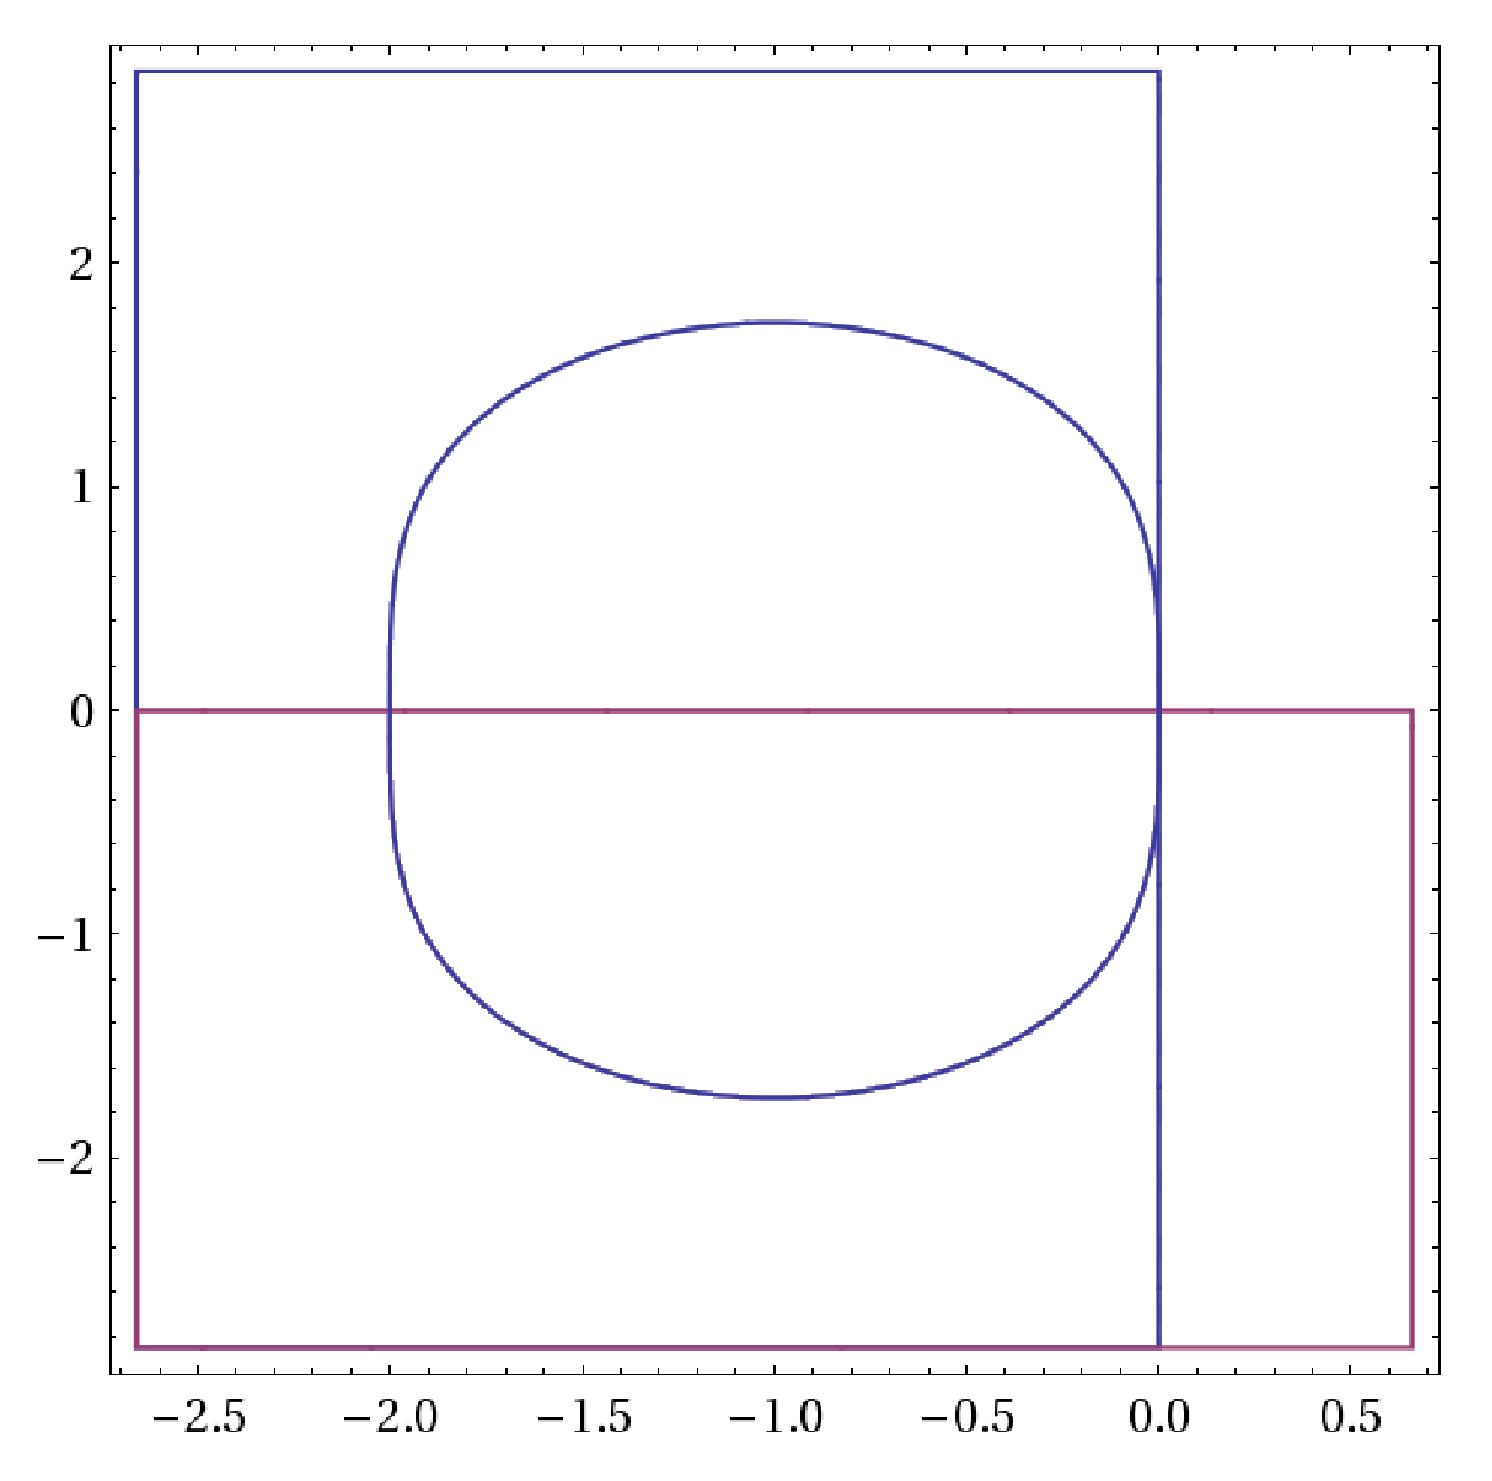
\includegraphics[width=0.6\textwidth]{../plots/eigenvalue/eigen1.eps}
%%   \caption{Two stage Runge-Kutta time marching scheme has the given contour for amplification factor, $\sigma = 1$ with the minimum real value being $\lambda \Delta t = -2$. The domain for second order upwind has a contour that is primarily dictated by the real values of CFL number. The minimum value is $-4\frac{u\Delta t}{\Delta x}$. Hence, that gives $CFL_{max}\leq 0.5$.}                
%%   \label{rk2}
%% \end{figure}
 
%% \begin{figure}
%%   \centering
%%   \includegraphics[width=0.6\textwidth, angle = -90]{../plots/smooth/Smooth.eps}
%%   \caption{Profiles of numerical solutions with (Superbee), and without flux limiting for a 100 control volume mesh size have been shown to demonstrate failure of flux limiting which is based on purely discontinuous solutions. ENO schemes prove useful for solution exhibiting mixed character.}                
%%   \label{smooth}

%% \end{figure}
 
%% \begin{figure}
%%   \centering
%%   \includegraphics[width=0.6\textwidth, angle = -90]{../plots/square/Square.eps}
%%   \caption{The Superbee flux limiting proves to be highly accurate in comparison to a non-limited scheme (for a 100 control volume mesh size) in solving a square wave.}                
%%   \label{square}
%% \end{figure}
 
 
%%     %% \begin{table}
%%     %%   \begin{center}
%%     %%     \begin{tabular}{|l | c | c | r|}
%%     %%       \hline
%%     %%       Mesh Size & Convergence Criteria & Iterations & $L_2$ Norm\\
%%     %%       \hline
%%     %%       10x10 & $10^{-8}$ & 120 & 0.00245705 \\
%%     %%       20x20 & $10^{-9}$ & 410 & 0.000638619\\
%%     %%       40x40 & $10^{-10}$ & 1629 & 0.000161223\\
%%     %%       80x80 & $10^{-11}$ & 6519 & 0.0000404044\\
%%     %%       \hline
%%     %%     \end{tabular}
%%     %%     \caption{Convergence beahviour of solutions using point Gauss-Seidel iterative scheme with over-relaxation (1.5)}
%%     %%     \label{table:norm}      
%%     %%   \end{center}
%%     %% \end{table}
    
%%     %% \item Poisson problem in pressure calculation for incompressible flows: The following equation was solved in a uniform grid  spanning the domain 1x1 in dimensions.
%%     %% \begin{equation}
%%     %%   \frac{\partial^2 P(x,y)}{\partial x^2} +   \frac{\partial^2 P(x,y)}{\partial y^2} = -{\left\{\frac{\partial u}{\partial x}\right\}}^2 +  2{\frac{\partial u}{\partial x}}{\frac{\partial v}{\partial y}} + {\left\{\frac{\partial v}{\partial y}\right\}}^2
%%     %% \end{equation}
    
%%     %% with the following velocity field and given boundary conditions.
%%     %% \begin{eqnarray}
%%     %%   u = x^3 - 3xy^2\\
%%     %%   v = -3x^2y + y^3
%%     %% \end{eqnarray}
%%     %% The source variation across the domain was simplified to the expression:
    
%%     %% \begin{equation}
%%     %%   S = -18{(x^2 + y^2)}^2
%%     %% \end{equation}
%%     %% \begin{table}
%%     %%   \begin{center}
%%     %%     \begin{tabular}{|l | c | r|}
%%     %%       \hline
%%     %%       Mesh Size & Convergence Criteria & Iterations\\
%%     %%       \hline
%%     %%       20x20 & $10^{-8}$ & 1002\\
%%     %%       40x40 & $10^{-8}$ & 2936\\
%%     %%       80x80 & $10^{-8}$ & 12238\\
%%     %%       \hline
%%     %%     \end{tabular}
%%     %%     \caption{Convergence behaviour of finite volume solutions of Poisson problem in pressure solved using point Gauss-Seidel scheme with over-relaxation 1.5}
%%     %%     \label{table:norm2}      
%%     %%   \end{center}
%%     %% \end{table}

    
%%     %% The ASME procedure for analysis of error and estimation of order was implemented for values of P($\frac{1}{2},\frac{1}{2}$) using 3 different meshes (20x20, 40x40 and 80x80) with constant grid refinement factor, r = 2 to simplify error estimation. With a maximum change per iteration of Gauss-Seidel taken as $10^{-7}$, the apparent order of the scheme was calculated as $\mathcal{O} \sim 1.75002$ and the solution was extrapolated to: $4.93743 \pm 2.35637 \times 10^{-5}$ taking iterations of 859, 2936, and 10173 respectively. The same scheme was run for a lower ($10^{-8}$) tolerance for the maximum solution change per solution, where the values obtained for P($\frac{1}{2},\frac{1}{2}$) stopped fluctuating. The apparent order for this scheme was improved to $\mathcal{O} \sim 1.972644$ and the extrapolated solution was $P = 4.9374927 \pm 1.633160 \times 10^{-5}$ i.e. a smaller error bound.
%% \newpage
%% \emph{Comments:}
%% \begin{itemize}
%% \item A phase lead is seen in the RK2 solution of the smooth function (unnoticeable in the discontinuous case due to other predominant errors). In the solution with 20 control volumes, a single time step (5\%) lead was noticed, and with 40 control volumes the solution leads by 3 time steps (3\%). 

%% \item  While implementing the Superbee flux limiting, as an experiment, the corner points in the $\Psi$ - r curve, were assigned to different parts of the curve. For example the point (r = 0.5, $\Psi$ = 1) can be assigned to curves $\Psi$ = 2r, or $\Psi$ = 1. To my disappointment, there is no significant change by changing where this corner point lies.

%% \item The odd trend of norms can be attributed to the irregular values of dt obtained for certain mesh sizes that make the errors in floating point propagate and finally cause the time marching to carry to a time greater than required (inspite of running the loop based on number of time steps rather than on total time, and implementing a dt/2.0 correction factor mechanism). These errors are not $1^{st}$ order due to this correction factor, but are $\approx$ 1.5 order. It is difficult to eliminate such error.
  
%% \item For the last few control volumes, the value of r for limiting schemes depends on cells outside the domain. To handle this, ghost cells were created that contained values of the first few control volumes. In effect, the values along the wave are tabulated beyond the mesh. This  maintains periodicity and also allows us to use limiting for the last 2 cells. To add a caption of glory to our success, the $L_2$ norm decreases as well!

%% \item The $L_2$ norms provide an interesting picture of numerical solution as tabulated in Table~\ref{table:norm2}. Although the non-limited flux evaluation is considerably accurate with smooth solutions, the Superbee clearly fails by losing slope near extrema (Fig.~\ref{smooth}). But the $L_2$ norm in the discontinuous Superbee solution is greater than that for the smooth Superbee solution (looks - Fig.~\ref{square} - can be deceiving)! Indeed, the limited solution fails near the step change (in the square wave solution) by a greater amount than its failure near extrema in smooth solutions.

%% \item A crucial change was made on your suggestion, to force the time loop to stop nearest to the final time, T (\emph(tFinal) in code). This was done by counting number of integer time steps rather than calculating floating-point time. This makes a huge difference, because with comparing floating point numbers although there is a considerable drop in error on doubling the number of control volumes, but, it is noticed that the error norm fluctuates as the cells are increased further. It is difficult to pin-point a number for control volumes, for which error decreases steadily with increasing cells. In fact, there seem to be two modes of errors that steadily decrease with increasing control volumes but have different orders ($1^{st}$ and $2^{nd}$) of magnitude. 

%% \end{itemize}

\end{document}
